\documentclass[11pt,letterpaper]{article}

% \documentclass{article}
%    \usepackage{amsmath}
%    \usepackage{amssymb}
%    \usepackage{amsfonts}
%    \usepackage{graphicx}
%    \usepackage[mathscr]{euscript}
%    %\usepackage{bbm}
%    \usepackage[margin=1.0in]{geometry}
%    \usepackage{hyperref}
%    \usepackage{comment}
%    %\usepackage{todonotes}

%    %\usepackage{simplewick}
%    \usepackage{slashed}
%    %\usepackage{undertildeMod}

%    %\usepackage{feynmp-auto}
%    %\usepackage{youngtab}
%    %\usepackage[vcentermath]{youngtab}

%\usepackage{tikz}

%    \usepackage{enumitem}

    \newcommand{\vectsym}[1]{ \vec{#1} }
    %\newcommand{\vectsym}[1]{ \overline{#1} }
    %\newcommand{\vect}[1]{\vectsym{\boldsymbol{#1}}}
%    \newcommand{\vect}[1]{\boldsymbol{#1}}
    \newcommand{\vect}[1]{\vectsym{#1}}

    \newcommand{\udd}[2][]{{{\mathrm{d}^{#1}} #2}}
    \newcommand{\ud}[2][]{{ \, \udd[#1]{#2} \,}}
    \newcommand{\dd}[3][]{\frac{\udd{^{#1} #2 }}{\udd{ {#3}^{#1} }}}
    \newcommand{\uDD}[2][]{{{\mathcal{D}^{#1}} #2}}
    \newcommand{\uD}[2][]{{ \, \uDD[#1]{#2} \,}}
    \newcommand{\fdd}[3][]{{  \frac{ {\delta^{#1}}#2}{\delta #3} }}
    \newcommand{\vdd}[3][]{{ \fdd[#1]{#2}{#3}  }}
    %\newcommand{\pdd}[2]{ \frac{ \partial{#1} }{ \partial{#2} } }
    \newcommand{\limint}[2]{ \int\limits_{#1}^{#2} }
    \newcommand{\limintf}[4]{\limint{#1}{#2}\frac{#3}{#4}}
    \newcommand{\limintd}[3]{ \int\limits_{#1}^{#2}{\udd{#3}\,} }
    %\newcommand{\intd}[1]{ \int{\udd{#1}} }
    \newcommand{\intd}[2][]{ \int{\udd[#1]{#2}\,} }
    \newcommand{\intD}[2][]{ \int{\uDD[#1]{#2}\,} }
    \newcommand{\intdf}[3][]{\int\frac{\ud[#1]{#2}}{#3}}
    \newcommand{\intdff}[4][]{\int\frac{\ud[#1]{#2}#3}{#4}}
    \newcommand{\limintdf}[5][]{\limint{#2}{#3}\frac{\ud[#1]{#4}}{#5}}
    \newcommand{\limintdff}[6][]{\limint{#2}{#3}\frac{\ud[#1]{#4}#5}{#6}}

    \newcommand{\unit}[1]{\,\widehat{ \boldsymbol{#1} }}
    \newcommand{\paren}[1]{{\left( #1 \right)}}
    \newcommand{\bparen}[1]{\Bigl( #1 \Bigr)}
    \newcommand{\bbparen}[1]{\Biggl( #1 \Biggr)}
    \newcommand{\brac}[1]{\left[ #1 \right]}
    \newcommand{\bbrac}[1]{\Bigl[ #1 \Bigr]}
    \newcommand{\bbbrac}[1]{\Biggl[ #1 \Biggr]}
    \newcommand{\cbrace}[1]{{ \left\{ #1 \right\} }}
    \newcommand{\bcbrace}[1]{{ \Bigl\{ #1 \Bigr\} }}
    \newcommand{\bmat}[1]{  \begin{bmatrix}  #1  \end{bmatrix}   }
    \newcommand{\pmat}[1]{  \begin{pmatrix}  #1  \end{pmatrix}   }
    %\newcommand{\inv}[1]{\frac{1}{ #1 } }
    \newcommand{\ddsq}[2]{\frac{\udd^2}{\udd{ #2 }^2} #1 }
    \newcommand{\nline}[1]{\noindent\textbf{ #1 }}
    \newcommand{\nprob}[2]{\nline{ #1 } \begin{align*} #2  \end{align*} }
    \newcommand{\neqs}[2][*]{\begin{align#1} #2 \end{align#1}}
    \newcommand{\abs}[1]{\left| #1 \right|}
    \newcommand{\flux}[0]{\Phi}
    \newcommand{\del}[0]{\nabla}
    \newcommand{\vdel}[0]{\vect{\del}}
    \newcommand{\eval}[2]{\biggl|_{#1}^{#2}\biggr. }
    \newcommand{\smeval}[2]{\Bigl|^{#1}_{#2}\Bigr. }
    \newcommand{\pd}[1]{\partial #1}
    \newcommand{\pdd}[3][]{\frac{\pd{^{#1} #2 }}{\pd{ {#3}
    %^{#1}
    }}}
    \newcommand{\ang}[1]{\left\langle #1 \right\rangle}
    \newcommand{\expon}[1]{ \,\mathrm{e}^{ #1 } }
    \newcommand{\emf}[0]{\varepsilon}

    \newcommand{\bfrac}[2]{ \brac{\frac{ #1 }{ #2 }} }
    \newcommand{\pfrac}[2]{ \paren{\frac{ #1 }{ #2 }} }
    \newcommand{\ptfrac}[2]{ \paren{\tfrac{ #1 }{ #2 }} }
    \newcommand{\vud}[2][]{ \ud{#1\vect{ #2 }} }

    \newcommand{\ee}[1]{\times10^{#1}}
    \newcommand{\un}[1]{\,\mathrm{ #1 }\,}
    \newcommand{\ans}[3]{\, #1 \ee{#2} \un{#3} }
    \newcommand{\qty}[3]{\paren{\, #1 \ee{#2} \un{#3} }}
    \newcommand{\smqty}[2]{\paren{\, #1 \un{#2} }}
    \newcommand{\smans}[2]{\, #1 \un{#2} }

    \newcommand{\basis}[1]{ \,\unit{\mathrm{e}}_{ #1 } }
    \newcommand{\q}[1]{q_{#1}}
    \newcommand{\bq}[1]{\,\unit{\mathrm{q}}_{#1}}
    \newcommand{\be}[1]{\basis{#1}}
    \newcommand{\bbe}[2]{\be{#1}\be{#2}}
    \newcommand{\bep}[1]{\be{#1}'}
    \newcommand{\vectc}[3]{ \vectcc{#1}{+#2}{+#3} }
    \newcommand{\vectcc}[3]{#1 \basis{x} #2 \basis{y} #3 \basis{z} }
    \newcommand{\tensor}[1]{#1}
    \newcommand{\tp}[0]{\mathrm{T}}%transpose
    \newcommand{\infsum}[1]{ \sum_{n=0}^{\infty}{#1} }
    \newcommand{\dualsum}[1]{\infsum{}\sum_{k=0}^{n}{#1}}
    \newcommand{\qeq}[0]{\overset{?}{=}}
    \newcommand{\res}[0]{\,\mathrm{res}}
    \newcommand{\resw}[1]{\res\paren{w,#1}}
    \newcommand{\Four}[1]{\mathscr{F}\left\{ #1 \right\}}
    \newcommand{\invFour}[1]{\mathscr{F}^{-1}\left\{ #1 \right\}}
    \newcommand{\Heav}[0]{\,\mathrm{H}}
    \newcommand{\heav}[0]{\Heav}
    \newcommand{\delt}[0]{\,\delta}
    \newcommand{\infint}[0]{\int_{-\infty}^{\infty}}
    \newcommand{\infintd}[1]{\infint\ud{#1}}
    \newcommand{\conv}[0]{\otimes}
    \newcommand{\scr}[1]{\mathscr{#1}}
    \newcommand{\Lap}[1]{\mathscr{L}\left\{ #1 \right\}}
    \newcommand{\invLap}[1]{\mathscr{L}^{-1}\left\{ #1 \right\}}
    \newcommand{\iif}{\quad \mathrm{if}\,}

    \newcommand{\pw}[2][cc]{\left\{ \begin{array}{#1} #2 \end{array} \right. }

    \newcommand{\pcos}[1]{\cos{\paren{#1}}}
    \newcommand{\psin}[1]{\sin{\paren{#1}}}

    \newcommand{\uu}[1]{\underline{#1}}
    \newcommand{\eq}[2][\notag]{\begin{equation}#1 #2 \end{equation}}
    \newcommand{\enum}[1]{\begin{enumerate} #1 \end{enumerate} }
    \newcommand{\bitem}[1]{\item[\textbf{#1}]}
    \newcommand{\bbitem}[2]{\item[\textbf{#1}] (#2)\,}

    \newcommand{\ffrac}[3][]{{ #1{\frac{#2}{#3}} }}
    \newcommand{\poissonbrac}[1]{ {\left\{ #1 \right\}} }
    \newcommand{\bars}[1]{{\left| #1 \right|}}
    \newcommand{\detmat}[1]{\begin{vmatrix} #1 \end{vmatrix}}
    \newcommand{\qtq}{\quad\to\quad}
    \newcommand{\qTq}{\quad\implies\quad}
    \newcommand{\opdot}[1]{\overset{\scriptscriptstyle \circ}{#1}}
    \newcommand{\opddot}[1]{\overset{\circ\circ}{#1}}

	\newcommand{\enumb}[1][]{\begin{enumerate}[#1]}
    \newcommand{\enume}{\end{enumerate}}

    \newcommand{\rr}{\vect{r}}
    \newcommand{\R}{\mathbb{R}}
    \newcommand{\Z}{\mathbb{Z}}

    \newcommand{\upperlower}[3]{{ {#1}^{#2}_{\phantom{2}#3} }}
    %\newcommand{\ul}[3]{\upperlower{#1}{#2}{#3}}
    \newcommand{\lowerupper}[3]{{ {#1}_{#2}^{\phantom{2}#3} }}
    %\newcommand{\lu}[3]{\lowerupper{#1}{#2}{#3}}

    \newcommand{\ket}[1]{{ \left | #1 \right \rangle }}
    \newcommand{\bra}[1]{{ \left \langle #1 \right | }}
    \newcommand{\bk}[2]{{ \left \langle #1 \middle | #2 \right \rangle }}
    \newcommand{\bok}[3]{{ \left \langle #1 \middle | #2 \middle | #3 \right \rangle }}
    \newcommand{\bo}[2]{{ \left \langle #1 \middle | #2 \right .}}
    \newcommand{\ok}[2]{{ \left . #1 \middle | #2 \right \rangle}}
    \newcommand{\kb}[2]{{ \ket{#1}\bra{#2} }}

    \renewcommand{\a}[1][\vphantom{\dagger}]{{a^{#1}}}
    \newcommand{\ad}{\a[\dagger]}
    \newcommand{\kk}{{k\vphantom{k'}}}
    \newcommand{\kp}{{k'}}
    \newcommand{\kpp}{{k''}}
    \newcommand{\comm}[2]{\brac{\,#1\,,\,#2\,}}
    \newcommand{\acomm}[2]{\cbrace{\,#1\,,\,#2\,}}
    \renewcommand{\L}{\scr{L}}
    \newcommand{\inv}{^{-1}}
    \newcommand{\norder}[1]{\,: #1 :\,}
    \newcommand{\obar}[1]{{ \overline{#1} }}
    \newcommand{\wick}[6][1]{{ \contraction[#1 ex]{#2}{#3}{#4}{#5} #2#3#4#5#6}}
    \newcommand{\sq}{^{\,2}}
    \newcommand{\fcn}[1]{{\,\mathrm{#1}\,}}
    \newcommand{\op}[1]{\widehat{#1}}
    \newcommand{\tr}{\fcn{tr}}
    \newcommand{\Tr}{\fcn{Tr}}
    \newcommand{\T}{\fcn{T}}

    \newcommand{\lra}{\leftrightarrow}
    \newcommand{\nothing}[1]{}
    \newcommand{\half}[1][1]{ {\frac{#1}{2}} }
    \newcommand{\thalf}[1][1]{ {\tfrac{#1}{2}} }
    \newcommand{\id}{ {\mathbf{1}} }
    \newcommand{\sigmab}{ {\bar{\sigma}} }
    \newcommand{\dg}{ {\dagger} }
    \newcommand{\pdg}{ {\vphantom{\dagger}} }
    \newcommand{\gr}[1]{ {\mathrm{#1}} }

    %\DeclareSymbolFont{bbold}{U}{bbold}{m}{n}
    %\DeclareSymbolFontAlphabet{\mathbbold}{bbold}

    \newcommand{\kd}[2]{{ \delta^{#1}_{#2}}}
    \newcommand{\kdu}[1]{{ \delta^{#1}}}
%    \newcommand{\Sl}[1]{{{ S_{#1}}}
%    \newcommand{\Su}[1]{{{ S^{#1}}}
%    \newcommand{\Smat}[4]{{{ (S_{#1#2})^{#3#4}}}
%    \newcommand{\kdg}[4]{{{ \kd{#3}{#1}\kd{#4}{#2}}}
%    \newcommand{\kdgg}[4]{{{ \kd{#4}{#1}\kd{#3}{#2}}}
%    \newcommand{\Smatd}[4]{{{ \kdg{#1}{#2}{#3}{#4}-\kdgg{#1}{#2}{#3}{#4}}}
%    \newcommand{\Smatdp}[4]{{{ \big(\Smatd{#1}{#2}{#3}{#4}\big)}}
%    \newcommand{\g}[1]{g_{#1}}
%    \newcommand{\gu}[1]{g^{#1}}
%····
    \newcommand{\ub}{\overline{u}}
    \newcommand{\vb}{\overline{v}}
    \newcommand{\gv}{\gamma^5}
    \newcommand{\gm}[1]{{\gamma^{#1} }}
%    \newcommand{\Tr}[1]{\,\mathrm{Tr}\brac{#1}}
    \newcommand{\ps}{\slashed{p}}
    \newcommand{\ks}{\slashed{k}}
    \newcommand{\pds}{\slashed{\pd}}
    \newcommand{\psib}{\bar{\psi}}

%    \newcommand{\ul}[3][]{#1^{#2\phantom{#3}}_{\phantom{#2}#3} }
    \newcommand{\ulul}[5][]{#1^{#2\phantom{#3}#4\phantom{#5}}
                            _{\phantom{#2}#3\phantom{#4}#5} }
    \newcommand{\symindBinU}[5]{ {#1}^{#2#3}{#1}^{#4#5} 
                                    + {#1}^{#2#4}{#1}^{#3#5}
                                    + {#1}^{#2#5}{#1}^{#3#4} }
    \newcommand{\symindBinL}[5]{ {#1}_{#2#3}{#1}_{#4#5} 
                                    + {#1}_{#2#4}{#1}_{#3#5}
                                    + {#1}_{#2#5}{#1}_{#3#4} }
    \newcommand{\gindBinU}[5]{ {#1}^{#2#3}{#1}^{#4#5} 
                                    - {#1}^{#2#4}{#1}^{#3#5}
                                    + {#1}^{#2#5}{#1}^{#3#4} }
    \newcommand{\gind}[4]{\gindBinU{g}{#1}{#2}{#3}{#4} }
    \newcommand{\tot}{\leftrightarrow}
    \newcommand{\diag}{\fcn{diag}}
    \newcommand{\itemb}{\begin{itemize}}
    \newcommand{\iteme}{\end{itemize}}

    \newcommand{\newQuestion}[2]{ \section*{Question #1 \textnormal{: #2 } } }
    \newcommand{\hc}{ {\text{h.c.}} }
    \newcommand{\ptext}[1]{\paren{\text{#1}}}

    \newcommand{\set}[1]{ \cbrace{#1} }
    \newcommand{\lie}[3][]{ {{\mathrm{#2}}_{#1}\paren{#3} } }

    \newcommand{\lag}{ {\mathcal{L}} }
    \newcommand{\Lag}{ \lag }
    \newcommand{\amp}[1][M]{ {\mathcal{#1}} }
    \newcommand{\Amp}[1][M]{ \amp[#1] }

    \newcommand{\p}{\vect{p}}

    \newcommand{\fig}[2][]{
	    \begin{figure}[#1]\begin{center}
		    #2
	    \end{center}\end{figure}
    }



% filename: PhysMan.tex

%% FOR Sans Serif UNCOMMENT THE FOLLOWING TWO LINES
%\usepackage[T1]{fontenc}
%\renewcommand*\familydefault{\sfdefault} %% Only if the base font of the document is to be sans serif
%% (To get normal Serif font again, comment the two lines)


%----------------------------------------------------------------
% Attempts at changing the font to sans serif style
%----------------------------------------------------------------

% http://www.tug.dk/FontCatalogue/sansseriffonts.html

%%\usepackage[light,math]{iwona}
%%\usepackage[T1]{fontenc}

%%\usepackage{cmbright}
%%\usepackage[T1]{fontenc}

% Works:
%\usepackage[T1]{fontenc}
%\renewcommand*\familydefault{\sfdefault} %% Only if the base font of the document is to be sans serif

%%\usepackage[default]{sourcesanspro}
%%\usepackage[T1]{fontenc}



%----------------------------------------------------------------
% Other style options
%----------------------------------------------------------------

\usepackage{fullpage}
\usepackage{graphicx}
\usepackage{amsmath}
\usepackage{amssymb} % Math symbols such as \boldsymbol

\usepackage{fancyhdr}
\pagestyle{fancy}
%\fancyfoot[C]{\thepage}
\usepackage[
%  margin=2.5cm,
  left=2.5cm, right=2.5cm,
  top=2cm, bottom=2cm,
  includefoot,
  footskip=30pt,
  headsep=1.25cm % Seperate header and main body by
		% headsep -- prevents first line from overlaying on top of header
]{geometry}

\usepackage[noams,squaren,Gray]{SIunits} % Standardizes quantity and SI unit spacing
\usepackage{soul} % for an underline macro that wraps
 \setul{0.2ex}{.4pt}% underline 0.2ex below contents
\usepackage{enumitem} % for enumerate options
\usepackage{verbatim} % Allows display of almost any sequence of symbols, printed in typewriter font; and provides comment environment
\usepackage[obeyspaces,spaces]{url} % Same as verbatim but allows line breaks and spaces
\usepackage{parskip}
 \setlength{\parindent}{0em}
 \setlength{\parskip}{2.2ex}

%\usepackage[compact]{titlesec}
%\titlespacing{\section}{0pt}{*1ex}{*0.5ex}
%\titlespacing{\subsection}{0pt}{*0}{*0}
%\titlespacing{\subsubsection}{0pt}{*0}{*0}
\usepackage{titlesec}
\titlespacing{\subsection}{0pt}{*2.5}{*0.1}



%----------------------------------------------------------------
% Macros
%----------------------------------------------------------------

% Scientific Notation and Units
% =============================

% scientific notation without units
\providecommand{\sn}[2]{ {#1} \mkern-1.5mu\times\mkern-3mu 10^{#2} }
% scientific notation with units
\providecommand{\snu}[3]{ \unit{\sn{#1}{#2}}{#3} }

% create compact or ``squished'' lists with sublists:
\newcommand{\squishlist}{
   \vspace{-2.2ex}
   \begin{list}{$\bullet$}
    { \setlength{\itemsep}{0pt}      \setlength{\parsep}{3pt}
      \setlength{\topsep}{3pt}       \setlength{\partopsep}{0pt}
      \setlength{\leftmargin}{1.5em} \setlength{\labelwidth}{1em}
      \setlength{\labelsep}{0.5em} } }
\newcommand{\squishend}{
    \end{list}  }

% struts for spacing in tabulars/tables
\newcommand{\tstrut}{\rule{0pt}{2.5ex}}
\newcommand{\bstrut}{\rule[-1ex]{0pt}{0pt}}
\newcommand{\Tstrut}{\rule{0pt}{2.9ex}}
\newcommand{\Bstrut}{\rule[-1.4ex]{0pt}{0pt}}


\usepackage{todonotes}
%\graphicspath{{../../imgs/6labs/6Alab/6Aexp6/}}
\graphicspath{{../../}}

\usepackage{hyperref}
\hypersetup{
    colorlinks=true,
    linkcolor=blue,
%    filecolor=magenta,      
%    urlcolor=cyan,
}

\usepackage{color}


\newcommand{\TODO}[2][inline,color=green!40]{{ \todo[#1]{#2} }}
\newcommand{\TODOg}[2][inline]{{ \todo[color=green!40,#1]{#2} }}
% Uncomment the following lines to compile document with no \TODO comments
% \renewcommand{\TODO}[2][]{}
% \renewcommand{\TODOg}[2][]{}

%\newcommand{\question}[2][]{{ \bf #2 }}
\newcommand{\question}[2][blue]{{ \textcolor{#1}{#2} }}

%\newcommand{\qq}[2][]{{ \question }}

\newcommand{\answer}[2][red]{{ \textcolor{#1}{#2} }}

\newcommand{\action}[2][]{ #2 }

\begin{document}

\fancyhead[C]{Physics 6A Lab \rule[-1ex]{0pt}{0pt}\(\mid\) Experiment 6}
%\fancyhead[C]{Physics 6A Lab \rule[+1ex]{5pt}{5pt}\(\mid\) Experiment 6}

\vspace{-5ex}
\part*{Overhauled Bicep Lab}

\TODO{See outline and future work at end of document}


\begin{comment}
%% Original revised version, and some notes
{{{

\subsection*{Notes from Allic}
\enumb
\item Main suggestion:  Cut content and make things inquiry-based
\item Just saying at the beginning something like ``This lab will be
	different.  We're expecting you to think about what steps to take,
	rather than just follow a recipe" has a big effect on the students'
	attitudes.  
	[Jared is not surprised by this, though he hadn't thought of doing it.]  
\enume

\subsection*{Warm up}
\subsubsection*{Meet the apparatus}
In this experiment, you'll attempt to understand torques and rotational
equilibrium using a model of the human arm.

Before we get into equations, take a moment to understand the equipment.  
	Fill in the blanks on the diagram below, from among the following choices:
	upper arm (humerus), elbow, forearm, hand, and biceps muscle.
\TODO{TODO -- Block out the labels in the picture of the apparatus,
	and replace with blanks -- 
	similar to a diagram one might fill in for a biology
	course.  Blanks include 
	upper arm (humerus), elbow, forearm, hand, and biceps muscle.}

\begin{figure}[h!]
	\centering
	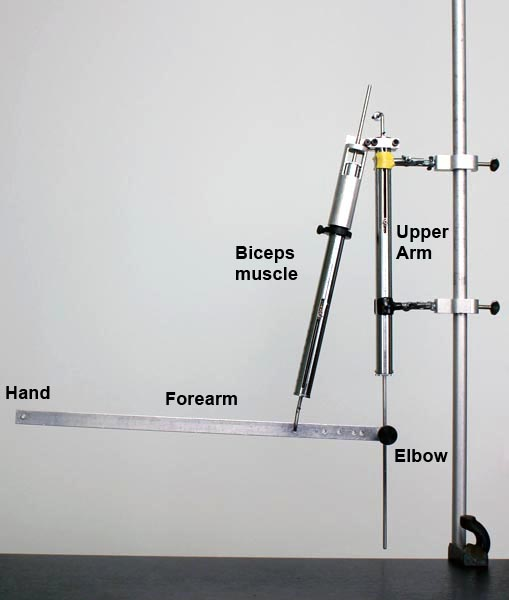
\includegraphics[width=0.6\textwidth]
	{{/imgs/6labs/6Alab/6Aexp6/6a-exp6_fig1_text_fix.jpg}}
\end{figure}

\subsubsection*{Get your head in the game}

Before making use of the apparatus,
let's do a brief warm up problem concerning \emph{torque}.

\TODO{TODO -- Now include an unrelated warm up problem dealing with
	static torque.  Possibly take this from UMD open source tutorials,
	or from tutorial books.}

\TODO{Maybe include a section getting students acquainted with the
	torque equation we're attempting to verify (relating bicep force to the
	force on the hand).}

\subsection*{Investigation}

Rather than telling you exactly what to do, 
in this lab we're going to allow you much more freedom to
investigate the physics behind this situation on your own.

}}}
\end{comment}

%\section*{Restart}

\section*{Introduction}

This lab will be different from the others you've done so far.
Rather than giving you explicit steps to follow,
we're providing you with a problem to investigate
and some hints on how to proceed.  
It will be something of a challenge to figure out how exactly to accomplish
each step, but this will be much more like doing science in the real world.


\subsection*{Warm up}
\subsubsection*{Warm up -- comments }
\itemb
	\item Assume students don't know anything about torque
		(it's very likely they won't know anything)
	\item Give activity which guides them through torque
	\item Possibly just take from open source tutorial
	\item Ok, open source tutorial requires them to do experiment that we don't
		have resources set up for (though we could relatively easily set them up)
\iteme

\subsubsection*{Warm up problems}

\TODO{A lot of these problems can be taken with minimal modification
	from the UMD open source 
	\href{https://www.dropbox.com/sh/i3iftgdflca6yj0/AAA37zsDuMN591__i-oPnjiSa/Suite\%20II/Instruction/Student_Materials/01_Torque/Tutorial_01_Torque.doc?dl=0}
		{tutorial on torque} 
		(and the 
		\href{https://www.dropbox.com/sh/i3iftgdflca6yj0/AABuUrEqKUU4ZvRvxi_cQLWYa/Suite\%20II/Instruction/Student_Materials/01_Torque/Tutorial_01_Homework.doc?dl=0}
		{corresponding HW assignment}
		) [click colored text for links], which focus on static torque ,
		especially on things like levers
}
\TODO[inline]{Note:  These questions would probably work better if
	the students could actually perform 
	some of these mini-experiments.
	I'm planning to talk to those in charge (not Marty, but others)
	to ask whether we have the materials needed to investigate 
	the balance of torques on a simple lever-fulcrum system
	(like the one in the 
	\href{https://www.dropbox.com/sh/i3iftgdflca6yj0/AAA37zsDuMN591__i-oPnjiSa/Suite\%20II/Instruction/Student_Materials/01_Torque/Tutorial_01_Torque.doc?dl=0}
	{open source tutorial activity}
	).
	{\bf Such an apparatus will not be available this quarter, but it may
	work for next quarter} -- 
	depending on the resources already in place.
}
\enumb
	\item Balancing weights on a ruler atop a fulcrum
		\enumb[label=\alph*.]
			\item Two equidistant weights on opposite side of pivot
			\item Double one weight's distance; ask how much weight needs to be
				added and to which side
		\enume
	\item Replace one of the weights with an arbitrary force pointing downward
	\item Replace arbitrary force with a cable at an angle 
		(positioned like bicep)
\enume

**Need to figure out how to introduce quantitative relations
\itemb
	\item $\tau \sim rF$ (for orthogonal force)
	\item $\tau \sim rF\sin\theta$
\iteme
Ideally, we'd have a simple experiment for them to figure out.
This is almost certainly possible for a future quarter. **

\subsection*{Procedure}
\TODO{Do we want them to measure upper arm force at all?
In the interests of time, likely not.}
We wish to investigate some of the forces involved with weight lifting.
Specifically, we'll examine the situation where you're holding a weight in your
hand, with your forearm being held horizontal.
We'll measure the forces experienced by both the biceps muscle
and the upper arm.

If you'd like, imagine yourself as a 
physical therapist or prostetic limb designer,
who wishes to combine physics with some 
general experimental design skills to determine 
some of the forces involved in lifting objects.

** Common sense warning about using reasonable values, 
making sure to keep everything but the thing you're measuring constant, etc.**

** Discussion about which variables are relevant.  Answer -- forces, distances,
angles. **

** Make sure to emphasize that we'll keep the forearm horizontal, 
to simplify things. **

\begin{enumerate}[label=\bf{\arabic*.}]

\item
Start by measuring the biceps force $B$ and the upper arm force $A$ 
for some fixed weight $H$ being held in the hand.

Then devise and carry out a procedure for measuring the forces $B$ and $A$ for
different weights $H$.  
\question{Make sure to explicitly write out the steps of the procedure.}
If you find you need to modify the procedure as you carry it out,
that's okay -- but be sure to change the written version to correctly
reflect the steps you really carried out.

After taking several measurements (you can choose a number which seems
reasonable), use your data to 
\question{extrapolate a relationship between the biceps
force $B$ and the weight $H$ in the hand.}
\question{Write a explicit formula for $B$ as a function of $H$.}
\emph{Hint:  In case this terminology is a bit unfamiliar, 
it might help to know that
$y(t) = \bparen{10\,\mathrm{m}} +\bparen{4.9\,\mathrm{m/s^2}}t^2$ 
is an example of an explicit formula 
for $y$ as a function of $t$ (for a certain physical situation).}
Make sure you specify the units of the quantities.

\item
Choose a new value for $H$ -- one that you haven't measured yet,
but that you are able to measure.  
Before you measure $B$, 
\question{use your model to predict the biceps force $B$ 
for this new value of $H$.}

** Ideally, first make a rough prediction of $B$ based only on neighboring data
points, but I probably won't add this due to time. **

Now use the apparatus to measure $B$ for this value of $H$.  
\question{How does it compare to the prediction from your model?  }
(Calculate the percent deviation.)
If the two values don't precisely agree, do
you think this is okay?  
\question{Do you think it tells us our model is wrong?}
Why or why not?

\end{enumerate}



\subsubsection*{Varying model parameters}
\TODO{TODO: Expand this prompt}
How does the bicep force change when we increase 
each of the following parameters:
\question{Fill in your own copy of the chart below, }
answering with ``increases'', ``decreases'', 
``stays constant'', or ``it depends''.
\vspace{.5cm}
\\
%\begin{tabular}{c||c|c|c}
\begin{tabular}{|c||c|c|c|}
	\hline
	Parameter change & Effect on $B$ & Effect of slope of graph &
	Effect on $y$-intercept of graph \\ \hline \hline
	$\uparrow R$ 
	& & & 
	\\ \hline
	$\uparrow r$ 
	& & & \\ \hline
	$\uparrow W$ 
	& & & \\ \hline
	$\uparrow \alpha$
	& & & 
	\\ \hline

\end{tabular}
\TODO{It will probably be difficult to describe what we mean by $\alpha$,
	and why it's important.}
\TODO{Consider having students come up with their own ideas of what parameters
	to vary.  Maybe only provide 3 lines.  Note that they might have trouble
	coming up with parameters other than $r$.  (Hopefully $r$ will be easy.)}




\begin{comment}
%% Section talking somewhat abstractly about models and asking for predictions.
	%% Likely difficult for students to comprehend, and likely will take too
	%% given the time constraints.
{{{
\subsubsection*{Extrapolate further}
The model you extrapolated from your data is a good description of the 
force $B$ on this apparatus for this setup.  But what if you change the
apparatus somehow?  For example, consider an apparatus which
is the same as yours, except the forearm bar is longer.
For the same value of the weight $H$ in the hand, 
would the corresponding biceps force $B$ change? 
In fact, it does: $B$ is larger for a larger value of $R$ 
(assuming all other parameters are left the same).
** Ideally ask them a question, to make sure they pay attention to this part.
**

In reality, you probably want a model of the biceps force that is valid 
beyond your specific apparatus.  
To do this, we'll try to determine the coefficients in your formula for 
$B(H)$ in terms of various parameters of your apparatus -- that is, in terms of
things you can actually measure!  
For example, one such parameter is the length of the forearm bar -- if you
change this parameter, the coefficients in the formular for $B(H)$ change.
\TODO{Subtelty -- three types of experimental parameters:  
	(1) independent/dependent variables, 
	(2) parameters which change model parameters, but not the form of the model
	(3) parameters which ``break'' the model 
		-- i.e., they change the form of the model.
	In this case, $r,R,\alpha,W$ are type (2), whereas the angle of the forearm
	to the horizontal is type (3).\\

	We might be able to get this across by giving them an extended worked
	example of another model -- for example, a simple static torque problem,
	like in the warm up.
}
}}}
\end{comment}

\subsubsection*{Understanding model parameters}
%\TODO{In the interest of time, it probably makes more sense to replace the
%previous section with this one.}
\TODO{
Ideally we'd have enough time to guide the students in deriving this formula,
but this isn't out main goal for the lab.  Hopefully we'll still give them some
intuition for the formula.
}

In a previous step above,
you experimentally determined a formula for the biceps force $B$ as a function
of the weight $H$ in the hand.  
%This formula included some coefficients (with units!).
Now we'll compare this model to the one the theory predicts.

It turns out that we can analyze the torques acting on the forearm
to determine a formula for $B$ vs $H$.  You actually have all the tools needed
to do this from the warm up exercises at the beginning of this lab, and we
encourage you to give it a try!  But in the interest of time, we'll just
provide you with the formula, which is as follows:
\begin{equation*}
	B = \paren{ H + \frac{W}{2} }\frac{R}{r\cos\alpha}
\end{equation*}

Given this theoretical model, 
can you determine what the theory predicts the coefficients appearing in
your formula for $B$ vs $H$ should be?  
\question{First write your answer in terms of symbols} 
(i.e., variables) only;
\question{then, plug in the values for those variables} from your apparatus, 
to determine the theoretical model coefficients.
How do these theoretical coefficients compare to your experimental model
coefficients?  
(\question{Calculate the percent difference} 
and \question{comment on how well they agree}.)

You just used a theoretical model to predict the values of your experimental
model coefficients.
Now, we'll look at the predictions the theoretical model makes on your data
itself.  
(This may seem similar to the previous step,
but there's actually a subtle difference.)
Hopefully, you noticed your data plot of $B$ vs $H$ was linear.
It turns out, we can use the theoretical model to predict what the slope and
$y$-intercept of that graph should be.
First, use the theoretical model to 
\question{predict the slope and $y$-intercept 
of your graph in terms of symbols only.}
Next, \question{plug in the actual parameter values 
from your experimental apparatus}
to get a numerical value for these parameters (with units!).
\question{How does this prediction compare 
with your actual slope and $y$-intercept?}

\TODO{Probably want to avoid making them do the same steps twice...}

\question{Do the theoretical predictions above agree 
with the predictions you recorded in the chart above},
regarding how the bicep force and linear equation parameters change when
increasing certain apparatus parameters?

You probably noticed some similarities between the previous steps.
Why do they seem so similar?  
Is there a relationship between the model parameters
and the slope and $y$-intercept of your graph?
\answer{Since this is a linear model, the model parameters are precisely
	the slope and the $y$-intercept of the graph.}




\section*{Outline}

Outline of steps up to this point so far
\itemb
	\item Warm up problems, introducing torque to the students for the first
		time
	\item (?) Warm up problems directly involving this apparatus
		\subitem Matching parts of apparatus to parts of body
		\subitem Short exercise with torque?  Maybe intuitive `if we increase
		$r$, what happens to bicep force?'
		\TODOg[]{TODO}
	\item Measure bicep force (and upper arm force) as a function of weight in
		hand.  Extrapolate equation from graph.
	\item Use the model for $B$ vs $H$ to make a prediction for a new value,
		and test the prediction.
	\item Try to understand coefficients in formula as functions of 
		physical parameters (e.g., lengths and weights) of the apparatus.
	\item TODO
\iteme

Remaining steps
\itemb
%	\item List parameters which must remain fixed for this model to have the
%		same form
%	\item List experimental parameters which can be changed within this model.
%		Realize the coefficients in
%		your formula are functions of these parameters.
	\item Reason physically how coefficients should change if each parameter is
		increased or decreased.
	\item Give them the full formala for $B(H;W,R,r,\alpha)$
	\item Perform some checks (both experimental and mathematical)
		to verify that this formula makes sense
	\subitem Understand that it is linear in certain variables
\iteme

\TODO{Note:  It's difficult to tell how much time this will take students, but
it's likely this is far too much content already.}




\end{document}
